Миний хувьд дадлагын 21 хоногийн хугацаа дахь сүүлийн долоо хоногт уг системийн мерчант вэб хэсэг дээр ажиллаж эхэлсэн ба гүйцэт биш ч тодорхой хэмжээнд системийн талаар судалгаа хийснээ хүргэж байна. Мөн уг систем дээр ажиллахын тулд нууцлалын гэрээ хийсэн учир дэлгэрэнгүй тайлбарлах боломжгүй. 

\quad \quad Oneline аппыг бодит амьдрал дээрх олон дэлгүүр байршдаг нэг барилга гэж үзэж болох ба та тус апп руу орсноор яг л нэг молл дотор дэлгүүр хэсэж байгаа юм шиг хамгийн түрүүнд Oneline дээр гэрээтэй дэлгүүрүүдийн жагсаалт харагдана. Уг байдлаараа монголд хөгжиж буй бусад  e-commerce-уудаас ялгаатай билээ. Харин миний ажилласан мерчант системийн гол үүрэг нь тухайн апп доторх дэлгүүрийг дэлгүүрийн эзэн буюу мерчант админ бүрэн удирддаг байх шаардлагатай.
\section{Хэрэглэгчийн шаардлага}
  \subsection{Хэрэглэгчид}
    \begin{itemize}
        \item Мерчант админ гэсэн ердөө ганц хэрэглэгчээс бүрдэнэ.
    \end{itemize}
	\subsection{Функционал хэрэглэгчийн шаардлагууд}
     \begin{itemize}
        \item Хэрэглэгч зөвхөн имэйлээр ирсэн холбоосоор нэвтэрдэг байх
        \item Хэрэглэгч өөрийн хаяг дээрээ олон дэлгүүр үүсгэх боломжтой байх
        \item Дэлгүүр бүр ажиллах цагийн хуваарьтай байх
        \item Дэлгүүр бүр cover болон icon зурагтай байх
        \item Дэлгүүр бүр бүтээгдэхүүний ангилалтай байх ёстой
        \item Бүтээгдэхүүний цуглуулга буюу коллекцийг үүсгэдэг байх
        \item Коллекц заавал cover болон icon зураг авдаг байх
        \item Хямдрал зарлах боломжтой байх
        \item Хямдралыг төрлөөр нь хувь, үнэ гэсэн хоёр хуваадаг байх
        \item Бүх бүтээгдэхүүн дээр хямдрал зарлах боломжтой байх
        \item Зөвхөн коллекци дээр хямдрал зарлах боломжтой байх
        \item Хэрэглэгчийн сервертэй харьцсан бүх үйлдэлд Toast-р хариу өгдөг байх
        \item Бүтээгдэхүүн үүсгэж болдог байх
        \item Бүтээгдэхүүн заавал нэг буюу түүнээс дээш зурагтай байх
        \item Бүтээгдэхүүний оруулж буй бүх зураг 1:1 хэмжээтэй байх
        \item Бүтээгдэхүүн заавал үнэтэй байх
        \item Мерчант дээр хуулагдаж буй бүх зураг alt таг авдаг байх
        \item Үүсгэсэн бүтээгдэхүүнээ засдаг байх
        \item Нүүр хэсэгт тухайн сонгосон дэлгүүрийн борлуулалтын статистикыг харуулдаг байх
        \item Нүүр хэсэгт тухайн сонгосон дэлгүүр дээрх барааны жагсаалт харагддаг байх
    \end{itemize}
  \subsection{Функционал бус шаардлага}
    \begin{itemize}
        \item Вэбсайт нь хэрэглэхэд хялбар байх
        \item Бүх хуудасны арын суурь өнгө ижил байх
        \item Responsive дизайнтай байх
        \item Бүтээгдэхүүн үүсгэх хэсэг хялбар байх
        \item Цагийн хуваарь болон дэлгүүрийн бусад мэдээлэл оруулахад ойлгомжтой байх
        \item Бүх хуудас тусламж авах хэсэгтэй байх
    \end{itemize}
\pagebreak
\section{Use Case диаграм}
	Мерчант вэб болон Oneline дээр хийгдсэн Use Case диаграм
\begin{figure}
	\centering
	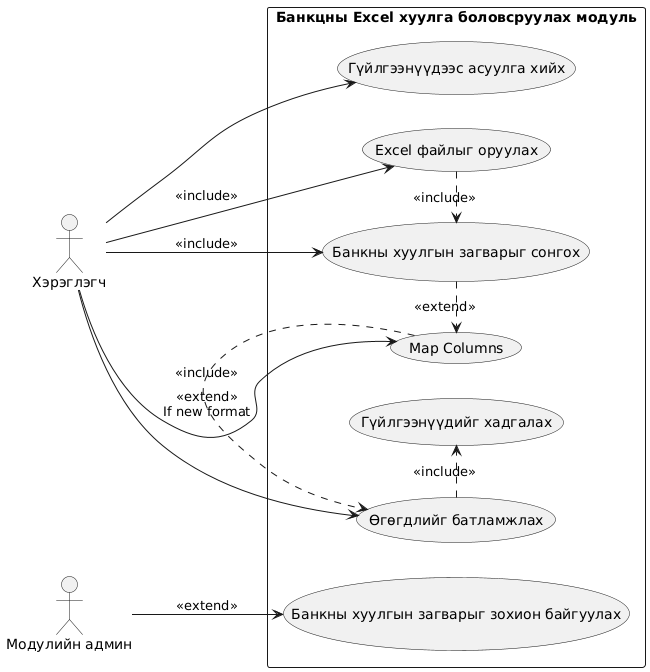
\includegraphics[width=15cm]{images/usecase-diagram.png}
	\caption{Use Case диаграм}
	\label{fig:form}
\end{figure}
